\section{Платформа для статистической обработки данных и работы с графикой Incanter}

Incanter - математический пакет для алгебраических и статистических расчётов на языке Clojure. Он был разработан под влиянием языка R, таким образом многие функции имеют структуру, похожую на аналогичные функции в R. Данный пакет является крупнейшим математическим пакетом для Clojure. Для реализации многих частей, таких как линейная алгебра, графика используются популярные Java библиотеки, например Parallel Colt (линейная алгебра, статистика), JFreeChart (библиотека для построение различных графиков).

Пакет включает в себя следующие основные модули:

\begin{itemize}
\item core - основные математические функцие, функции для работы с матрицами и векторами;

\item charts - функции для построение и отображения различных графиков и гистограмм, также есть возможность создания динамических графиков;

\item stats - функции для произведение статистических расчётов;

\item distributions - функции для моделирование различных видов распределения случайной величины;

\item latex - функции для отображения математических формул, применяется для добавление подписей к графикам;

\item mongodb - функции для работы с базой данных MongoDB;
\end{itemize}

\subsection{Примеры}

Работа с матрицами

\begin{minted}{clojure}

  (def a (matrix [[1 2 3] [4 4 6] [7 8 9]])) ; matrix 3x3

  (def b (matrix [1 2 3])) ; vector of 3 elements

  (solve a) ; finds inverse matrix of a

  (solve a b) ; solves system a x = b

  (mmult a a) ; multiplies a by itself

\end{minted}

Построение графиков

\begin{minted}{clojure}
  (view (histogram (sample-normal 1000)))
\end{minted}

\centerline{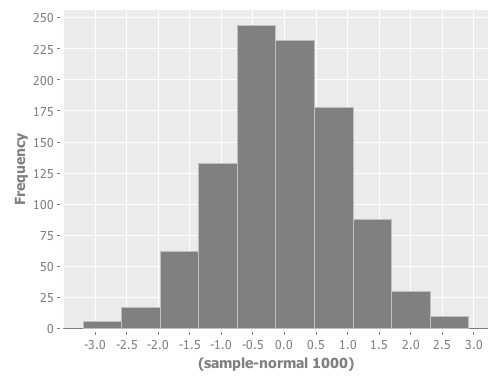
\includegraphics[width=\textwidth,height=\textheight,keepaspectratio]{histogram_example}}

\begin{minted}{clojure}
  (view (function-plot sin -10 10))
\end{minted}

\centerline{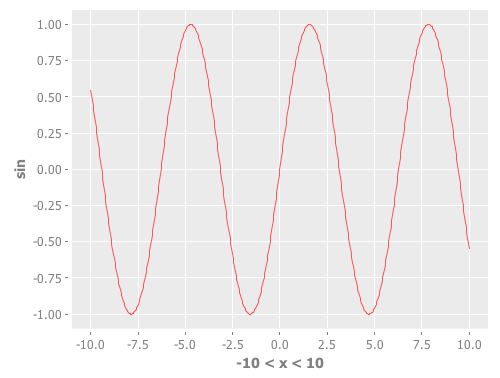
\includegraphics[width=\textwidth,height=\textheight,keepaspectratio]{function_plot_example}}

%%% Local Variables:
%%% mode: latex
%%% TeX-master: "../document"
%%% End:
